\documentclass[11pt]{article}

\usepackage{amsmath, amssymb, amsthm}
\usepackage{tikz}

\theoremstyle{plain}
\newtheorem{thm}{Theorem}[section]
\newtheorem*{thm*}{Theorem}
\newtheorem{prop}[thm]{Proposition}
\newtheorem{lem}[thm]{Lemma}
\newtheorem*{lem*}{Lemma}
\newtheorem{dfn}[thm]{Definition}
\newtheorem{cor}[thm]{Corollary}
\newtheorem{claim}[thm]{Claim}
\newtheorem{conj}[thm]{Conjecture}
\newtheorem{ques}[thm]{Question}
\newtheorem*{rem}{Remark}


\oddsidemargin  0pt
\evensidemargin 0pt
\marginparwidth 40pt
\marginparsep 10pt
\topmargin 0pt
\headsep 10pt
\textheight 8.2in
\textwidth 6.4in
\renewcommand{\baselinestretch}{1.1}

\newcommand{\codeg}{\text{codeg}}
\newcommand{\BBE}{\mathbb{E}}
\newcommand{\BFP}{\mathbf{P}}
\usepackage{amsmath}
\usepackage{amsthm}
\usepackage{amssymb}
\usepackage{mathtools}
\usepackage{hyperref}
\usepackage{url}





\usepackage{graphicx}
\usepackage{caption}
\usepackage{subcaption}

\def\eQb#1\eQe{\begin{eqnarray*}#1\end{eqnarray*}}
\def\eQnb#1\eQne{\begin{eqnarray}#1\end{eqnarray}}
\providecommand{\e}[1]{\ensuremath{\times 10^{#1}}}
\providecommand{\pb}[0]{\pagebreak}
\DeclarePairedDelimiter\ceil{\lceil}{\rceil}
\DeclarePairedDelimiter\floor{\lfloor}{\rfloor}

\newcommand{\E}{\mathrm{E}}
\newcommand{\Var}{\mathrm{Var}}
\newcommand{\Cov}{\mathrm{Cov}}

\def\Qb#1\Qe{\begin{question}#1\end{question}}
\def\Sb#1\Se{\begin{solution}#1\end{solution}}


\newtheoremstyle{quest}{\topsep}{\topsep}{}{}{\bfseries}{}{ }{\thmname{#1}\thmnote{ #3}.}
\theoremstyle{quest}
\newtheorem*{definition}{Definition}
\newtheorem*{theorem}{Theorem}
\newtheorem*{lemma}{Lemma}
\newtheorem*{question}{Question}
\newtheorem*{preposition}{Preposition}
\newtheorem*{exercise}{Exercise}
\newtheorem*{challengeproblem}{Challenge Problem}
\newtheorem*{solution}{Solution}
\newtheorem*{remark}{Remark}
\usepackage{verbatimbox}
\usepackage{listings}
\usepackage{mathrsfs}
\date{}
\title{\vspace{-0.7cm}
Diff Geo II: Problem Set III}

\author{
Youngduck Choi 
\thanks{Department of Mathematics, Courant Institute of Mathematical Sciences, 
yc1104@nyu.edu; If you find an error and want to share with me, 
you can reach me via email.
}}

\begin{document}

\maketitle

\begin{abstract}
This work contains solutions for the problem set III.
\end{abstract}


\begin{question}[1-1]
\hfill
\begin{figure}[h!]
  \centering
    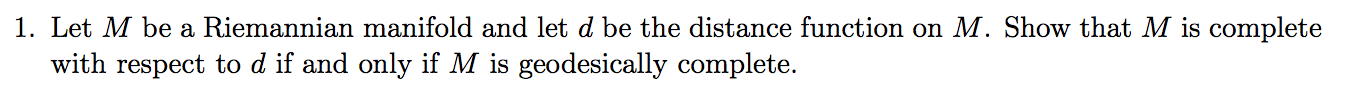
\includegraphics[width=0.7\textwidth]{dg-s4-p1.png}
\end{figure}
\end{question}
\begin{solution} \hfill \\
Firstly, it is necessary to assert that the Riemmanian manifold must be connected
in this context;
otherwise, there can be two points $x,y \in M$, such that $d(x,y) = \infty$
where $d$ is the standard Riemmanian distance, 
as the infimum of an emptyset by convention
is $\infty$. Therefore, $d$ does not even satisfy
the property of a metric, hence we cannot make sense of the "completeness" of
the metric space of Riemmian distance, induced by the Riemmanian metric. If we
assume connected, since connected manifolds are path connected, and doing replacement
of a piecewise continuous path to piecewise smooth path, if necessary, we can 
gurantee the well-definedness of the Riemmnian distance as a metric function on a 
set. Now, we proceed to prove the statement. 
Suppose $M$ is complete, but not geodesically complete. Then, we can choose a unit
speed geodesic $\gamma:[0,b) \to M$ such that it does not extend to $[0,b+\epsilon)
$ for any $\epsilon > 0$. Let $\{a_n\}$ be an increasing sequence, limiting to $b$,
and set $\{ q_n = \gamma(a_n)\}$. By construction,
\eQb
d(q_n,q_m) &\leq& |a_n - b_m|
\eQe 
for any $n,m$, so $\{q_n\}$ is Cauchy, and via completeness $q_n$ converges to some
point $q \in M$. Now, choose $N$ be a uniformly normal neighborhood of $q$, and
$\delta >0$ be chosen that the geodesic $\delta$ ball at each point contains $N$,
and for convenience we can assume without loss of generality that $\delta < b$. 
Now, for $n$ large enough $a_n > b - \delta$, so every geodesic starting at 
$q_n$ exists for at least time $\delta$ for $n$ large enough,
via the property of normal neighborhoods. 
This, in particular, implies that there is a geodesic $\gamma^*$ such that 
$\gamma^*(0) = q_n$ and $\dot{\gamma^*}(a_n)$ for some $n$ large enough. By
uniqueness $\tilde{\gamma}(t) = \sigma(a_n + t)$ is an extension of
$\gamma$ upto $a_n + b - \delta > 0$, which contradicts the minimality of $b$. Now,
for the converse, suppose $M$ is geodesically complete. From class, we know that
geodesically complete is equvivalent to exp defined on all of the tangent bundle.
Also, by Hopf-Rinow proven in class, we have that there exists a minimal geodesic
for any two points on $M$, which we denote as property $(*)$.
Fix $p \in M$, and set $M_n = \exp_p(\overline{B_n(0)})$
for all $n$. These are compact, as its an image of compact set of a continuous map. 
From (*), we see 
\eQb
\bigcup_{k=1}^{\infty} M_n = M
\eQe 
Now, let $\{x_n\}$ be cauchy in $M$. This implies that the Riemmanian distance is bounded
on $\{x_n\}$, and since Riemmanian distance agrees with the distance in $T_pM$, through
exp map, we can find $k$ large enough such that $\{x_n\} \subset M_k$. Since, compactness
implies completness in a general metric space, we see that $x_n$ converges to
some $x \in M_k \subset M$, and we are done. \hfill $\qed$ 
\end{solution}

\newpage

\begin{question}[1-2]
\hfill
\begin{figure}[h!]
  \centering
    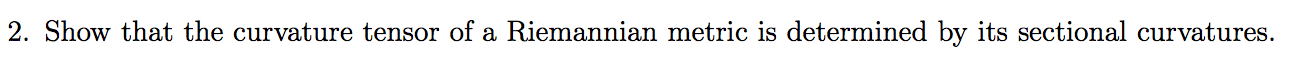
\includegraphics[width=0.7\textwidth]{dg-s4-p2.png}
\end{figure}
\end{question}
\begin{solution} \hfill \\
We here assume the well-definedness of the sectional curvature, $K$: it does not
depend on the choice of the pair of vectors
of the tangent space at the point. Now, fix $p \in M$. We claim that
If $K = 0$ at $p$, then $R = 0$ at $p$. Firstly, let $v,w \in T_p(M)$. Then, 
if $v$ and $w$ span a non-degenerate plane then, $<R_{vw}v,w> = 0$. Otherwise,
there is a technical lemma, which asserts that any pair of vectors is a 
limit of non-degenerate vectors. By multilinearity, and continutiy of 
$<R_{vw}x,y>$ on $T_p(M)^4$, we see that $<R_{vw}v,w> = 0$. We now claim that
$R_{vw}v = 0$. By polarization identity,
\eQb
<R_{v,w+x}v, w+x> &=& <R_{vw}v,w> + <R_{vx}v,w> + <R_{vw},x> + <R_{vx}v,x>
\eQe 
and by the previous remark, and symmetry of pairs,
\eQb
<R_{vw}v,x> = 0
\eQe
for any $x \in T_pM$. Now, again by polarization,
\eQb
R_{v+x,w}(v+x) &=& R_{vw}x + R_{xw}v + R_{vw}x + R_{xw}x
\eQe 
and by the previous remark, and skew-symmetry in subscripts, 
\eQb
R_{vw}x = R_{wx}v
\eQe
for all $x \in T_{p}M$. Hence, by first Bianchi identity, we see that 
\eQb
R_{vw}x = 0
\eQe
for any $x \in T_{p}M$, so $R = 0$ at $p$. Now, suppose $F$ is a multilinear 
on $T_p(M)^4$. and has symmetries properties enjoyed by $<R_{vw}x,y>$. Then, 
from the previous remark, we see that $R$ is completely characterized by
\eQb
K(v,w) &=& \dfrac{F(v,w,v,w)}{<v,v><w,w,> - <v,w>^2},
\eQe
for any $x,y,v,w \in T_p(M)$,
as taking the difference and applying the previous remark shows that the difference is
0. \hfill $\qed$
\end{solution}

\newpage

\begin{question}[1-3]
\hfill
\begin{figure}[h!]
  \centering
    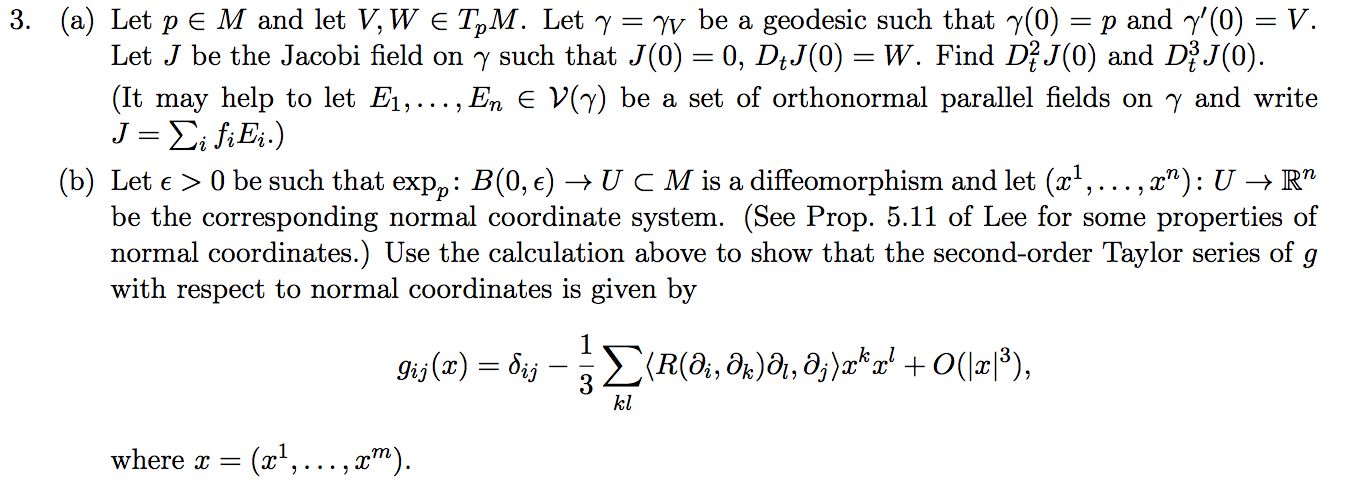
\includegraphics[width=0.7\textwidth]{dg-s4-p3.png}
\end{figure}
\end{question}
\begin{solution} \hfill \\
\textbf{(a)} We compute 
\eQb
<J,J>' &=& 2<J',J> \\
<J,J>'' &=& 2<V'',V> + 2<V',V'> \\
&=& 2<R(\gamma',J)\gamma',J> + 2<J',J'> \\
<J,J>''' &=& 2<R(\gamma',J)'\gamma',J> + 6<R(\gamma,J)\gamma',J'> \\
<J,J>''' &=& 8<R(\gamma',J)',\gamma',J'> + 2<R(\gamma',J)'',\gamma',J> + 
6<R(\gamma',J)\gamma',J''>.  \\
\eQe
Plugging in $t = 0$, first and third terms disappear and 
\eQb
<J,J>''(0) &=& <w,w> \\
<J,J>''''(0) &=& 8<R(v,w)v,w>. 
\eQe
We will use that 
\eQb
<V(t),V(t)> = <w,w>t^2 + \dfrac{1}{3}<R(v,w),v,w>t^4 + O(t^5).
\eQe


\smallskip

\noindent 

\textbf{(b)} Let $w \in T_pM$, and consider the geodesic $\gamma(t) = \exp_p(tw)$,
and let $c$ be a curve in $T_pM$ such that $c(0) = w$ and $\dot{c}(0) = v$, which
can be chosen by setting $c(s) = w +sv$. Then, set
\eQb
\Gamma(t,s) = \exp_{p}(tc(s)).
\eQe
Observe that $\gamma$ is a geodesic variation of $\gamma$, with the variation field
over $\gamma$, is given by,
\eQb
V(t) &=& \Gamma_s(t,0) = d(\exp_p)_{tw}(tv) = td\exp_{p}(tw)(v).
\eQe
Then, $V(0) = 0$, and $V'(0) = \Gamma_{st}(0,0) = \Gamma_{ts}(0,0)$. Furthermore, 
$\Gamma_s(t,0) = \exp_p(tv)$ and differntiating with respect to $t$ and taking value 
at $t = 0$ yields $v$. Hence,
\eQnb
d(\exp_p)(tw)(v) = t^{-1}V(t) \label{eq:3-b-1}
\eQne 
where $V$ is the Jacobi field along $\gamma(t) = \exp_p(tw)$ with $V(0) = 0$ and
$V'(0) = v$. Now, apply the above result with each $e_1,...,e_n$ orthonormal basis
of $T_pM$, to obtain the corresponding Jacobi fields $J_1,...,J_n$. Then, by a property
of normal coordinates, and~\eqref{eq:3-b-1},
\eQnb
\partial_j(\exp_p(tw)) = d(\exp_p)_{tw} e_j = t^{-1}J_j(t) \label{eq:3-b-2} 
\eQne
for all $j$. Hence,
\eQnb
g_{jk}(\exp_{p}(tw)) &=& <\partial_j(\exp_p(tw)), \partial_k(\exp_p(tw)> \nonumber \\
&=& t^{-2}<J_i,J_k>(t) = t^{-2}(t^{2}<e_j,e_k> + \dfrac{t^4}{3}<R(w,e_j)w,e_k> + 
 O(t^5)) \label{eq:3-b-3} \\
&=& \delta_{jk} + \dfrac{t^2}{3} <R(w,e_j)w,e_k> + O(t^3) = 
\delta_{jk} + \dfrac{1}{3} R_{ijkl} x^ix^l + O(t^3) \label{eq:3-b-4}  \\
&=& \delta_{jk} - \dfrac{1}{3} R_{iklj}x^kx^l + O(t^3);
\eQne 
where~\eqref{eq:3-b-3} holds by~\eqref{eq:3-b-2} and~\eqref{eq:3-b-4} holds via
$w = t^{-1}x$ substitution.  


\end{solution}

\end{document}
